% Compiles with a stock TeX Live: pdflatex main; bibtex main; pdflatex main; pdflatex main
% Two-column, self-contained (no external conference class required).
% To target a specific venue, swap \documentclass for {IEEEtran} (conference)
% or {acmart} and adjust the title block accordingly.
\documentclass[10pt,twocolumn]{article}

\usepackage[utf8]{inputenc}
\usepackage[T1]{fontenc}
\usepackage{lmodern}
\usepackage[margin=0.75in]{geometry}
\usepackage{amsmath,amssymb}
\usepackage{booktabs}
\usepackage{cite}
\usepackage{microtype}
\usepackage[hidelinks]{hyperref}
\usepackage{xcolor}
\usepackage{tikz}
\usetikzlibrary{positioning,shapes.geometric}

\setlength{\columnsep}{0.28in}

\title{\textbf{[Draft] In Search of Sustainable Pace in Agentic Coding
and Orchestration}}

\author{
  Marinos Prevenios\\
  \small Independent Research\\
  \small\texttt{marinos.prevenios+research@gmail.com}
  \and
  Daphne Tsolissou\\
  \small Independent Research\\
  \small\texttt{daphne.tsolissou+research@gmail.com}
}
\date{}

\begin{document}
\twocolumn[
\begin{@twocolumnfalse}
\maketitle
\begin{abstract}
\noindent
This work presents a \emph{self-regulating feedback mechanism} that gives each
software engineer a research-grounded, \emph{private} view of supervision load
over time and surfaces an individualized \emph{sustainable pace}: the personal
operating band in which throughput and supervision quality remain in balance.
The method turns session data already recorded by local agentic-coding tools into
a longitudinal behavioural index. It decomposes load into three axes: Concurrent
Operational Demand Load (CODL), an Interruption Index, and a Closure Deficit.
These axes draw on working-memory capacity, supervisory-control fan-out,
interruption and attention-residue research, prospective-memory monitoring
costs, the cognition of unfulfilled goals, and the Job Demands--Resources model.
The resulting index is an early behavioural proxy for multitasking overload, not
a diagnosis of stress or burnout. It is deliberately limited to agent
interaction, which competes with an engineer's other work for finite daily
cognitive capacity. An open-source implementation performs all processing
locally, scores daily load against each engineer's personal history, and supports later
population calibration through anonymized exports that users share manually.
The metric thresholds are priors drawn from adjacent human-factors literature
and require validation in a representative population. Because the axes measure
properties of the human operator rather than of software engineering itself,
similar load may surface in other professions as agent supervision spreads
beyond engineering.
\end{abstract}
\vspace{1.5em}
\end{@twocolumnfalse}
]

\section{Introduction}
Coding assistants based on large language models increasingly operate in
concurrent sessions. The human role shifts from direct code production toward
\emph{supervision}: dispatching tasks, switching between agents, judging
partial results, and re-engaging with failed or dormant threads. The closest well-studied
analogue is supervisory control of multiple semi-autonomous vehicles, where a
single operator's performance is known to collapse non-linearly past a personal
``fan-out'' limit, often \emph{before} the operator consciously registers
overload~\cite{cummings2008,crandall2007,sheridan1992}.

Three properties make this load hard to see from the individual's standpoint. First, it is
\emph{concurrent}: holding multiple open agent conversations fills up human working
memory, whose capacity for independent items is famously small (about
four)~\cite{cowan2001}. Second, it is \emph{interruption-dense}: switching
between agents and reacting to failures fragments attention and leaves residue
that slows the resumed task~\cite{mark2008,mark2005,leroy2009,wickens2008}.
Third, it is \emph{closure-poor}: agentic work spawns many mental loops that are parked
and resumed rather than finished in one sitting, and each cold resumption reloads
decayed context at a cost that grows with the gap~\cite{monk2008,altmann2002}.
Demands that exceed recoverable resources are the mechanism of burnout in the Job
Demands--Resources model~\cite{demerouti2001}, and chronic load without
recovery (not isolated peaks) is what damages people over
time~\cite{mcewen1998,sonnentag2010}.

This is not a speculative concern. For AI-assisted coding specifically, a
growing body of peer-reviewed work finds that effort does not disappear under
assistance but \emph{shifts} from writing into verification and oversight:
software engineers spend roughly half their session time in assistant-specific
states (verifying suggestions, deferring thought, prompt-crafting, and
editing)~\cite{mozannar2024}; software engineers given an AI assistant write less secure
code while being \emph{more} confident it is secure~\cite{perry2023}; and
professional engineers show automation complacency and rising reliance over the
course of a single task~\cite{qian2024}. A mixed-methods survey of $442$
software engineers links GenAI adoption to burnout through intensified job
demands~\cite{feng2026}. Crucially, this load is hard to read from the inside:
in a randomized trial, experienced software engineers were slowed by $\approx 19\%$ when
allowed AI tooling yet believed it had sped them up~\cite{metr2025}. This
perception--reality gap is echoed in longitudinal telemetry~\cite{sergeyuk2026} and
large-scale software engineer surveys~\cite{so2025}.

These dynamics are compounded by the natural incentive to maximise throughput:
running the most sessions in parallel, cycling through more orchestration
pipelines, spending the most tokens per unit of time. The developer community
describes this pattern as \emph{tokenmaxxing}. The logic appears sound; tokens
are cheap and engineer attention is not. But the perception--reality gap above
reverses the conclusion: if the marginal agent session consumes attention faster
than it produces verified output, adding more of them is counterproductive. The
operating point that maximises \emph{useful} throughput lies somewhere inside the
inverted-U performance curve, not at the maximum-concurrency end, and locating
it requires a signal the engineer can act on.

The goal of this work is to provide that signal: a research-grounded,
\emph{private} picture of each software engineer's supervision load over time,
scored against \emph{their own} historical baseline and a personally-discovered
operating optimum. The method does not claim to measure stress, to diagnose
burnout, or to replace validated subjective instruments. It makes an
otherwise-invisible \emph{behavioural} quantity visible and actionable.

The aim is \emph{not} to make people use these tools less. They are
genuinely helpful, and throttling agent use to drive the index down would
forfeit that value and miss the point. The aim is to help each software engineer
navigate their own \emph{sustainable pace}: the personal operating band in which
the quality of supervision and the cognitive overhead of sustaining it stay in
balance. The framing parallels Kanban's use of work-in-progress limits,
which cap the number of concurrent items not to slow delivery but to maximise
\emph{flow} and protect a sustainable pace~\cite{anderson2010,beck2000}: a
limit set too low wastes a capable system, one set too high overloads it, and
the right value is specific to the system and discoverable only by observing
it. Concurrent agent supervision is the same control problem with the
work-in-progress limit relocated into a single human's attention, where it is
ordinarily invisible. Making the load observable turns that limit into an
adjustable parameter; the personal optimum (\S\ref{sec:optimum}) operationalises
it as a target band to steer toward rather than a ceiling to stay under. The
result is a self-regulating feedback mechanism: the score provides the demand
signal, the optimum makes the target band discoverable from the engineer's own
data, and the engineer closes the loop by adjusting their agent load toward the
concurrency where speed and supervision quality are jointly sustained.

The intended use is \emph{individual self-assessment}: a working engineer gauging
their own multitasking and exhaustion over time. As an early behavioural proxy,
the index offers a warning to investigate rather than a clinical diagnosis
(\S\ref{sec:threats}). Its scope is intentionally limited to the engineer's
\emph{interaction with coding agents}, not the whole working day. Writing and
supervising code is only one part of a role that also includes design, code
review, debugging, coordination, and planning. All of these activities draw on
the same finite pool of attention and working memory. The index measures only
the agent-supervision demand imposed on that shared pool, but that partial
coverage is still informative. An extreme agent-interaction load suggests that
either little capacity remains for other work or the quality of that work,
including the AI-assisted development itself, may suffer. The index is thus better read
as \emph{how much of a finite attention budget agent-supervision consumed} than
as a tally of activity; what is left for everything else is an inference it
invites, not a quantity it observes.

The contributions offered in this work are:
\begin{enumerate}
  \item A decomposition of agent-supervision taskload into three axes with
  explicit thresholds (\S\ref{sec:method}).
  \item An \emph{engagement-weighted} concurrency measure that distinguishes
  actively-supervised sessions from background ``cooking'' ones, grounded in
  prospective-memory and unfulfilled-goal research (\S\ref{sec:codl}).
  \item An open-source implementation that
  serves as a working proof of concept~\cite{acsrepo} (\S\ref{sec:impl}).
  \item A deliberately adversarial treatment of the construct itself
  (\S\ref{sec:threats}) and a validation roadmap with falsifiable predictions
  (\S\ref{sec:validation}).
\end{enumerate}

\section{Background and Related Work}
The proposed index connects established findings about concurrent attention,
interruption, recovery, and unfinished goals with emerging evidence from
AI-assisted software development.

\paragraph{Concurrency and working memory.} Cowan's reconsideration places the
capacity of focal attention for independent chunks at roughly
four~\cite{cowan2001}; this serves as the reference point past which tracking
parallel agents should degrade.

\paragraph{Supervisory control and fan-out.} The human-supervisory-control
tradition models an operator dividing attention across automated
processes~\cite{sheridan1992}. ``Fan-out'' is the number of robots an operator
can effectively manage; it is bounded by \emph{neglect time} (how long a process
runs unattended) and \emph{interaction time}. An agent's \emph{attention
demand} is the fraction of operator time it
consumes~\cite{cummings2008,crandall2007}. The engagement weighting in
\S\ref{sec:codl} translates this framing into the proposed index.

\paragraph{The supervisory shift across professions.} Software is not the first
field where automation converts a practitioner from a producer into the
supervisor of several semi-autonomous producers. The recurring lesson is
that the human's load rises rather than falls: the more capable the automation,
the more demanding and safety-critical the residual monitoring role
becomes~\cite{bainbridge1983}. Cockpit automation moved pilots from flying to
monitoring, trading manual effort for vigilance decrement and ``automation
surprises''~\cite{wiener1980}. Anesthesiology makes the fan-out explicit: one
anesthesiologist medically directs several concurrent operating rooms, and
higher staffing ratios (more rooms overseen at once) are associated with worse
patient outcomes~\cite{burns2022}. En-route air-traffic-control workload scales
with the number of aircraft a single controller holds, and decision-support
automation is introduced precisely to raise that count, with workload as the
binding constraint~\cite{loft2007}. Cross-sectional imaging multiplied the
images per study by orders of magnitude, leaving each radiologist interpreting
an image every few seconds across a shift~\cite{mcdonald2015}. In translation,
machine-translation post-editing turns the translator into a high-throughput
reviewer of generated text~\cite{krings2001}, whose output is measurably flatter
and more source-interfered than translation from scratch
\cite{toral2019}. Across professions the same pattern that agent-assisted
programming produces recurs: automation does not subtract work so much as
convert it into the steering and review of more parallel output than one person
previously handled. Once that fan-out passes a personal ceiling, the operator's
load rises while the scrutiny each output receives declines
(\S\ref{sec:codl}).

\paragraph{Interruption and attention residue.} Interrupted work is completed
faster but at the cost of higher stress and effort~\cite{mark2008}. Fragmented
work and frequent external switches are costly~\cite{mark2005}, with residue
from an unfinished task impairing the next~\cite{leroy2009}. Cross-modality
or cross-tool switches are more costly than within-tool ones~\cite{wickens2008}.

\paragraph{Demands, recovery, and the optimum.} The Job Demands--Resources model
frames burnout as ``demands outstripping recoverable
resources''~\cite{demerouti2001}. Allostatic-load theory stresses that
\emph{sustained} activation, not peaks, causes the most harm~\cite{mcewen1998}; and
psychological detachment in off-hours predicts next-day
well-being~\cite{sonnentag2007,sonnentag2010}. Performance follows an inverted-U
in arousal/load~\cite{yerkes1908}, the ``flow channel'' between boredom and
anxiety~\cite{csikszentmihalyi1990}, motivating a \emph{personal optimum} rather
than a fixed ceiling.

\paragraph{Open mental loops and monitoring costs.} A backgrounded task carries
some cost without demanding full attention. Unfulfilled goals remain
active in memory and intrude on unrelated tasks until the goal is closed or a
concrete plan is made~\cite{masicampo2011}; and maintaining a pending intention
while doing other work measurably slows that ongoing task, the
prospective-memory ``monitoring cost,'' on the order of 15--20\%\ of
baseline~\cite{smith2003}.

\paragraph{AI-assisted coding and software engineer cognition.} A young but fast-growing
empirical literature studies these tools directly, and it is what makes the
present concern concrete. AI assistance shifts effort
toward verification: software engineers spend $\approx 51.5\%$ of session time in
suggestion-specific states~\cite{mozannar2024}, and merely \emph{informing}
software engineers that code is LLM-generated raises their measured NASA-TLX
workload~\cite{tang2024}. Over-reliance is demonstrated rather than
hypothesised: a ``false sense of security'' among users who write
less secure but more confidently-trusted code~\cite{perry2023}, and automation
complacency among professional engineers~\cite{qian2024}. The interaction
is also bimodal, alternating fast \emph{acceleration} with slow, validation-heavy
\emph{exploration}~\cite{barke2023}. Burnout now has its first peer-reviewed
anchor in a Job Demands--Resources analysis of GenAI
adoption~\cite{feng2026}. What this literature still largely lacks is direct,
longitudinal, AI-vs-no-AI measurement of cognitive load in everyday professional
work~\cite{sergeyuk2026}; this index approaches that gap from the opposite
direction: an objective behavioural signal computed continuously from real
sessions on the software engineer's own machine, rather than a one-off laboratory
measurement.

\paragraph{Review volume and output quality.} Greater review volume can reduce
review quality. In human code inspection the
\emph{review rate} (lines examined per hour) is the dominant controllable
determinant of how many defects a review removes: defect-removal effectiveness
falls sharply once the rate climbs past roughly two hundred lines an
hour~\cite{kemerer2009}. This is a domain instance of the general
speed--accuracy trade-off, in which faster processing is bought with a higher
error rate~\cite{wickelgren1977}. Supervising several agents concentrates more
generated output into the same reviewing hours and splits the attention each
output receives, raising the effective review rate precisely as the load axes
(\S\ref{sec:method}) rise. The expected consequence is not a busier
employee but thinner scrutiny per output. A heavy supervision load may therefore
degrade the quality of the very work it produces, compounding the
over-reliance findings above~\cite{perry2023,qian2024}.

\paragraph{What the index is \emph{not}.} The validated instrument for subjective
workload is NASA-TLX~\cite{hart1988}; for diagnosed burnout it is the Maslach
Burnout Inventory~\cite{maslach1981}. This index is neither; it is an objective
behavioural proxy, and \S\ref{sec:threats} treats the gap as the central threat.
The method records an optional, coarse felt-stress self-report, but only as a
calibration criterion against which the objective index can be checked, not as
part of the index itself. These boundaries motivate the explicitly provisional
behavioural construction that follows.

\section{Method}\label{sec:method}

The pipeline from raw logs to a daily score is summarised in
Figure~\ref{fig:pipeline}; the remainder of this section defines each stage.

\subsection{Data model}
The input consists of session transcripts that coding tools already store locally. A
pluggable adapter maps each tool's log into a common interface of typed events
(user message, assistant message, tool use, tool result/error) with UTC
timestamps. Events are reduced to per-day
\emph{stream} records: one stream is one session on one day, summarised by its
first/last event timestamps $[a_s,b_s]$, per-type counts, the multiset of
the user's own message timestamps $U_s$, and the timestamps of any errored tool
results. All processing is local; nothing is
transmitted over the network (\S\ref{sec:impl}).

\begin{figure}[t]
\centering
\scriptsize
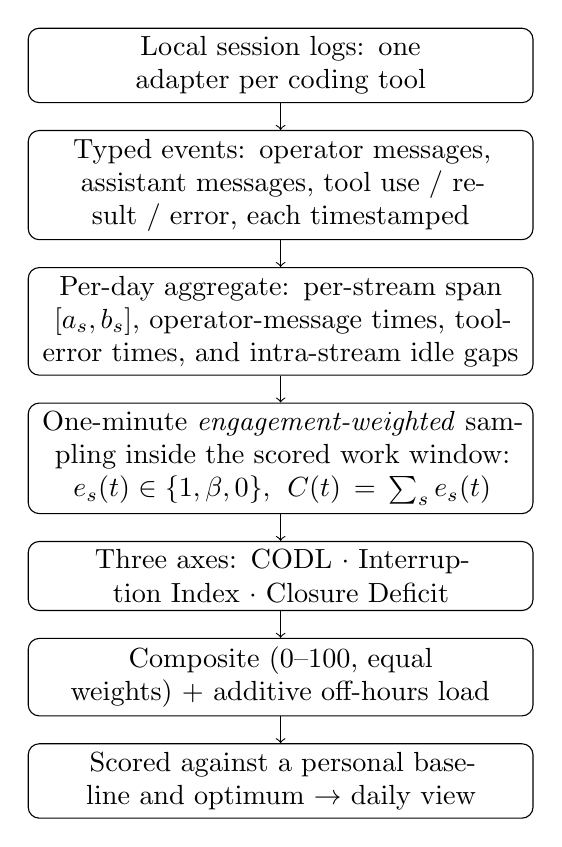
\begin{tikzpicture}[
  node distance=3.4mm,
  pbox/.style={draw, rounded corners, align=center, inner sep=3pt,
               text width=62mm, minimum height=6mm},
  every path/.style={draw, ->}
]
\node[pbox] (logs) {Local session logs: one adapter per coding tool};
\node[pbox, below=of logs] (events) {Typed events: operator messages, assistant messages, tool use / result / error, each timestamped};
\node[pbox, below=of events] (agg) {Per-day aggregate: per-stream span $[a_s,b_s]$, operator-message times, tool-error times, and intra-stream idle gaps};
\node[pbox, below=of agg] (sample) {One-minute \emph{engagement-weighted} sampling inside the scored work window: $e_s(t)\!\in\!\{1,\beta,0\}$,\; $C(t)=\sum_s e_s(t)$};
\node[pbox, below=of sample] (axes) {Three axes: CODL $\cdot$ Interruption Index $\cdot$ Closure Deficit};
\node[pbox, below=of axes] (comp) {Composite (0--100, equal weights) $+$ additive off-hours load};
\node[pbox, below=of comp] (score) {Scored against a personal baseline and optimum $\rightarrow$ daily view};
\path (logs) -- (events);
\path (events) -- (agg);
\path (agg) -- (sample);
\path (sample) -- (axes);
\path (axes) -- (comp);
\path (comp) -- (score);
\end{tikzpicture}
\caption{From logs to a daily score.}
\label{fig:pipeline}
\end{figure}

\subsection{Work window}
Before the event streams can be compared across days, the method establishes a
personal work window. The axes are computed inside a daily window
$W=[w_0,w_1]$ \emph{inferred per
operator}: $w_0=\lfloor p_{10}\rfloor$ and $w_1=\lceil p_{90}\rceil$ are the
$p_{10}$ and $p_{90}$ of the local-time hours at which the operator sends
messages, floored and ceiled \emph{outward} to whole hours so the band is never
narrower than the percentile span. The message hours are pooled over the baseline
window, and the resulting stable band is applied to \emph{every} calendar day. A
degenerate or empty band falls back to the cold-start default below.
The window is therefore individual to the operator rather than a property of
the experiment. No assumption is made about which dates are working days; any
date can contain work. ``Work'' is whatever falls
inside the operator's own inferred hours, on any date; engaged activity past
the end of those hours (or implausibly far before their start) is the
off-hours signal of reduced \emph{recovery}, again on any date (the boundary's asymmetry
is defined with the composite below). An early start within the early-start
grace before $w_0$ extends the scored window's lower bound to that first engaged
minute, so an early morning is credited on the three axes as ordinary in-window
work. A manual band may be configured to override inference; before enough data accrues
($<5$ distinct dates of activity) a conventional 09:00--19:00 local band serves
as a cold-start default. The scored window is sampled at one-minute resolution;
let $T$ be the set of sample instants.

Off-hours is thus defined relative to the operator's own agent-interaction
hours, not the calendar: the index measures the \emph{additional} strain of
agentic coding, not total workload or work--life balance. It follows that the
index has no notion of a \emph{rest day}: a seven-day-a-week operator with
consistent hours registers no off-hours signal. This is a scope boundary
rather than a defect.

\subsection{Engagement-weighted CODL}\label{sec:codl}
A simple concurrency count treats a stream as one continuously active locus
across its whole $[a_s,b_s]$ span. This over-counts in two ways: a session left
running while the operator is away reads identically to one being actively
juggled, and a session whose tool was closed during a long silence and relaunched
later reads as if it stayed open across the gap. Two refinements address these in
turn, a live-run restriction on \emph{when} a stream is open and an engagement
weight on \emph{how much} an open stream costs.

A stream is \emph{live} only across its run intervals. The session logs record
activity, not process liveness, so a sufficiently long silence is treated as a
closed and later relaunched process: an idle gap of
at least a cutoff $\theta$ (default $3$\,h) splits $[a_s,b_s]$ into separate runs,
and the dead span between them counts as no open session. Shorter gaps stay
inside one run, where the tool plausibly remained open and a process would still
be alive. Let $L_s$ be the union of stream $s$'s run intervals.

Within the live set, each stream is weighted by \emph{engagement} at each
instant. Let $g$ be a foreground grace window (default $5$ minutes) and
$\beta\in[0,1]$ a background weight. The instantaneous weight of stream $s$ at
time $t$ is
\begin{equation}
e_s(t) =
\begin{cases}
1 & \text{if } \exists\,u\in U_s:\; 0 \le t-u \le g \\[2pt]
\beta & \text{else if } t \in L_s \\[2pt]
0 & \text{otherwise.}
\end{cases}
\end{equation}
That is, a session counts fully only within $g$ of one of the operator's own
messages (\emph{foreground}, actively driven); otherwise, while live, it is
``cooking'' in the background at weight $\beta$; and across a closed-tool gap, or
before it opened or after it closed, it counts nothing. Weighted concurrency and
the two CODL summaries are
\begin{multline}
C(t)=\sum_{s} e_s(t),\quad
\overline{\mathrm{CODL}}=\frac{1}{|T|}\sum_{t\in T} C(t),\\
\mathrm{CODL}^{\star}=\max_{t} C(t).
\end{multline}
A raw headcount $H(t)=\sum_s \mathbf{1}[t \in L_s]$ and its peak
$\max_t H(t)$ are retained as a descriptive ``sessions open at once,'' counting a
session only while its tool was plausibly open, but the \emph{scored} quantities
use the weighted form.

\paragraph{Choosing $\beta$.} A background locus is neither cost-free nor
equivalent to a foreground locus.
A session left ``cooking'' while the operator attends elsewhere is precisely the
\emph{out-of-the-loop} regime of human supervisory control: the operator
periodically lets a semi-autonomous process run unattended and must re-engage to
judge or correct it. That literature is consistent on three points that bear
directly on $\beta$. Monitoring a process while it runs autonomously is not idle time but
\emph{effortful}, and sustained monitoring is itself a source of
stress~\cite{warm2008}; remaining out of the loop degrades situation awareness
and imposes a cost when control is resumed~\cite{endsley1995,eriksson2017}; and
under concurrent load operators systematically under-monitor automation
(complacency), so the divided-attention cost is real rather than
hypothetical~\cite{parasuraman2010}. Together, these findings ground a positive residual
cost ($\beta>0$) in a regime far closer to agent supervision than the laboratory. For the
\emph{magnitude}, a number is still borrowed: the prospective-memory cost of holding
a pending intention, $\approx$15--20\%\ of ongoing-task capacity~\cite{smith2003},
with unfulfilled goals consuming working memory until closed~\cite{masicampo2011},
and the supervisory-control ``attention demand'' fraction on the operator
side~\cite{crandall2007}. The value $\beta=0.20$ is adopted, the top of that band,
to favour a stronger residual-load estimate. $\beta$ and $g$ are
configuration parameters, not hard-coded constants, so the assumption is auditable
and tunable (\S\ref{sec:validation}).

\subsection{Interruption Index}\label{sec:interruption}
Where CODL captures sustained concurrent demand, the Interruption Index captures
discrete events that redirect attention.
Tool calls \emph{within} an active session are not counted: while an agent
works, the operator is in a ``waiting'' state in which attention can legitimately
detach, so counting each call would inflate the rate by orders of magnitude and
violate the standard definition of an interruption as an unscheduled event
demanding immediate attention. Two events do pull attention: a tool
\emph{error} (the operator may need to intervene) and a \emph{cross-stream
start} (a new session opened while another was active, forcing a switch and leaving
attention residue~\cite{leroy2009}). With $E^{\mathrm{win}}$ the number of tool
errors logged within the work window, $X$ the in-window cross-stream starts,
and $h$ the window length in hours,
\begin{equation}
I = \frac{1.5\,E^{\mathrm{win}} + 3.0\,X}{h}.
\end{equation}
The weights encode a higher expected cost for cross-stream switches than for
tool errors, following the relative costs in the interruption
literature~\cite{mark2008,mark2005,wickens2008}; the normalization
ceiling is $10$/hour, well above the field baseline of a working-sphere switch
roughly every $\approx$11~minutes ($\approx$5/hour) observed in knowledge
work~\cite{gonzalezmark2004}.

\subsection{Closure Deficit}\label{sec:closure}
Interruptions capture the switch itself; the Closure Deficit captures the later
cost of returning. A loop that the operator cannot finish in one sitting remains
open, and resuming it is not free: a suspended goal's activation decays over
the gap and must be reconstructed on return~\cite{altmann2002}. The cost of
that reconstruction rises with how long the task was suspended~\cite{monk2008}.
In the programming domain specifically, resuming an interrupted task reliably
incurs a context-reconstruction tax: only a small fraction of interrupted
sessions resume coding within a minute, and fewer still resume without first
navigating to rebuild context~\cite{parnin2011}. Closure, conversely, is a
recovery resource~\cite{sonnentag2007}, and the tendency to return to interrupted
tasks is a robust behavioural regularity, even as the older claim that open tasks
are better \emph{remembered} fails to replicate~\cite{ghibellini2025}. The
method therefore measures the day's \emph{resumption load}: how much the operator
re-entered parked sessions, weighted by how cold each had gone.

A \emph{resume} is a true-idle gap in a single session's event timeline whose
length falls in the band $[\tau,\theta)$: a span during which no event of any kind
(user message, model message, or tool call) was recorded and whose resuming event
is the operator or model re-engaging rather than a single long-running tool call
returning its result. A span that ends only because a tool returned is the agent's
own working time, not a parked loop, and is excluded. Below the lower bound
$\tau$ ($=30$\,min by default) the loop was paused, not suspended. At or above
the upper bound $\theta$ (the same close cutoff that bounds a live run,
\S\ref{sec:codl}, $3$\,h by default), the method treats the break as recovery
rather than a resume: the pickup begins a fresh sitting instead of reloading a
loop presumed to have remained active. A gap spanning a calendar day is treated
the same way. The cost of one resume saturates with the gap length $r$,
\begin{equation}
\sigma(r) = \min\!\Big(1,\ \frac{r}{\Delta}\Big),
\end{equation}
where $\Delta$ ($=120$\,min) is the horizon past which the context is treated as
fully cold. Under this linear-then-flat duration--cost curve, a $150$-minute gap
is no costlier than a two-hour gap~\cite{monk2008,altmann2002}. With
$\mathcal{R}$ the set of resumes whose pickup instant falls inside the work
window $W$, the daily ceiling is $K=4$. This is a loose working-memory anchor:
more than about four fully cold reloads in a day suggests movement among more
contexts than working memory comfortably holds~\cite{cowan2001}. The resulting
metric is
\begin{equation}
\mathrm{ClosureDeficit} =
\operatorname{clip}\!\Big(\frac{1}{K}\sum_{r\in\mathcal{R}}\sigma(r),\ 0,\ 1\Big).
\end{equation}
A value of $0$ denotes that every loop was closed in one sitting, and
the axis is defined on every active day, requiring no configuration. It is
\emph{undefined} (omitted as data, not scored) only on a day
with no activity at all. The thresholds $\tau$, $\Delta$, and $K$ are
citation-anchored modeling priors, not values fitted to felt load; all three are
configurable.

This axis is built from per-session resume \emph{events}, not from the concurrency
time-series $C(t)$, so it is independent of the CODL shape by construction: two
days with identical $C(t)$ (hence identical $\overline{\mathrm{CODL}}$) receive
different deficits if one parked-and-reloaded its loops while the other ran them to
completion in a sitting; this is information $C(t)$ cannot carry. The gap is, however,
a \emph{proxy} for a
parked loop and not a certainty (\S\ref{sec:threats}): a long \emph{autonomous}
agent turn is correctly excluded because it is not idle, but stepping away with a
session still mid-turn is not distinguished from a true suspension. And the
supporting laboratory evidence~\cite{monk2008,altmann2002} measured \emph{short}
interruptions, on the order of seconds to a minute; even the sub-$\theta$ gaps
this axis scores extrapolate well beyond that regime, with the field study of
interrupted programming~\cite{parnin2011} as the closest in-domain bridge.

\subsection{Composite}\label{sec:composite}
Each axis is normalized to $[0,1]$ and blended with equal weights. The Closure
Deficit is defined on every active day (\S\ref{sec:closure}), so all three axes
contribute to the score on every day with activity:
\begin{multline}
\mathrm{Composite} = \frac{100}{3}\bigg(
\min\!\Big(1,\tfrac{\overline{\mathrm{CODL}}}{5}\Big) +
\min\!\Big(1,\tfrac{I}{10}\Big) \\
+\ \mathrm{clip}(\mathrm{ClosureDeficit},0,1)
\bigg).
\end{multline}
The composite is written as a weight-normalised mean (the blend divided by the
sum of the weights) so that a calibrated, non-equal weight vector still maps onto
the same $0$--$100$ scale (\S\ref{sec:validation}); under the equal weights above
it reduces to the simple mean of the three axes. A day with no activity at all
defines none of the axes and is not scored.
The CODL ceiling is set to $5$, one above Cowan's $\approx 4$ capacity limit.
A day operating \emph{at} the working-memory boundary therefore scores $0.8$
(the warning band) rather than saturating the axis at $1.0$.
Off-hours work then adds an \emph{additive} load to this base. Let $o$ be the
day's off-hours \emph{engaged} minutes: one-minute instants during which the
operator was actively driving a session (within the foreground grace $g$ of one
of their own messages, \S\ref{sec:codl}) that fall \emph{after} the end of $W$,
or more than an early-start grace $g_{\mathrm{e}}$ (default $3$ hours) \emph{before} its
start. The reported composite is
\begin{equation}
\mathrm{Composite}^{\!*} = \min\!\big(100,\ \mathrm{Composite} + 30\cdot\min(1, o/90)\big).
\end{equation}
Three design choices matter here. First, the toll is \emph{additive}, not
multiplicative: off-hours work always counts, so a day worked \emph{entirely}
outside the window (zero in-window base) still scores a positive composite,
which a multiplicative form would wrongly leave at zero. The sum is capped at
$100$, so the increment raises the composite only to the extent that the
in-window base leaves headroom below the ceiling. If the in-window axes already
saturate the score, off-hours minutes produce no further movement. Second, $o$ is anchored
to \emph{interaction}, not stream liveness: a background session left running
while the operator is away contributes nothing; only measured engagement with
the agent outside the operator's own hours counts (e.g.\ waking
in the night to check on a run). Third, the boundary is \emph{asymmetric}:
every engaged minute past the window end counts, while minutes before its start
count only beyond the early-start grace. The recovery literature locates the
cost in failure to \emph{disengage} at the day's end~\cite{sonnentag2007};
beginning somewhat earlier than usual is an ordinary schedule shift rather than
a recovery deficit. Penalising it would classify routine schedule variation as
reduced recovery. Such an early start is scored as ordinary in-window work, with only
the off-hours toll waived, so a morning begun ahead of the usual hour still
registers on the three axes. The grace is bounded so that genuinely nocturnal engagement stays
visible: small-hours work (e.g.\ 01:30 against a noon start) lies far beyond
any plausible early start and counts in full. The
inferred band $W$ is the operator's norm; engaged work past it (or
outlier-early before it) is treated as a deviation from that norm. Like the
background weight $\beta$, the magnitudes (the $+30$-point toll saturating at
$90$ engaged minutes, and the $3$-hour grace) are explicit priors, not fitted
values (\S\ref{sec:threats}), grounded in disengagement as a recovery
resource~\cite{sonnentag2007}.
Equal weights are the explicit \emph{null hypothesis}: there is
no evidence that one axis dominates felt load, and stating that is preferred
to fitting weights to a single user's data. Replacing equal weights with empirically
calibrated ones is a primary validation target (\S\ref{sec:validation}).
The reference implementation colors and ranks each day against the
operator's \emph{own} percentile distribution (p50/p75/p90) computed over
active days in the baseline window, never a population norm, reinforcing
that only relative movement within one person's history is interpreted
(see the corresponding caveat in \S\ref{sec:threats}).

\subsection{Personal optimum and recovery}\label{sec:optimum}
Performance follows an inverted-U with load~\cite{yerkes1908,csikszentmihalyi1990}.
Historical workdays are bucketed by $\overline{\mathrm{CODL}}$ (width $0.5$).
Each bucket is rewarded for low average Closure Deficit and penalised for average
off-hours engagement; the midpoint
of the best bucket is reported as the operator's individual ``flow channel''
target, a line on the chart rather than a ceiling. This target is the
empirically discovered analogue of a personal work-in-progress limit: the
concurrency band at which the operator sustains the most closure, found by
observation rather than assumed. Because the Closure Deficit
is independent of concurrency (\S\ref{sec:closure}), this scoring term is not a
function of the very $\overline{\mathrm{CODL}}$ used to form the buckets, so
the optimum is not circular: it asks which load band \emph{actually} closed the
most loops, rather than rediscovering the load band with the least concurrency.
It requires at least 14 active days to stabilise, below which the report shows
``calibrating.''
Off-hours activity (on any date) is flagged because sustained load without
detachment, not peaks, predicts harm~\cite{mcewen1998,sonnentag2007,sonnentag2010}.

\subsection{Method revision: the paper as adversarial reviewer}\label{sec:reflexive}

\begin{figure}[t]
\centering
\scriptsize
\resizebox{\columnwidth}{!}{%
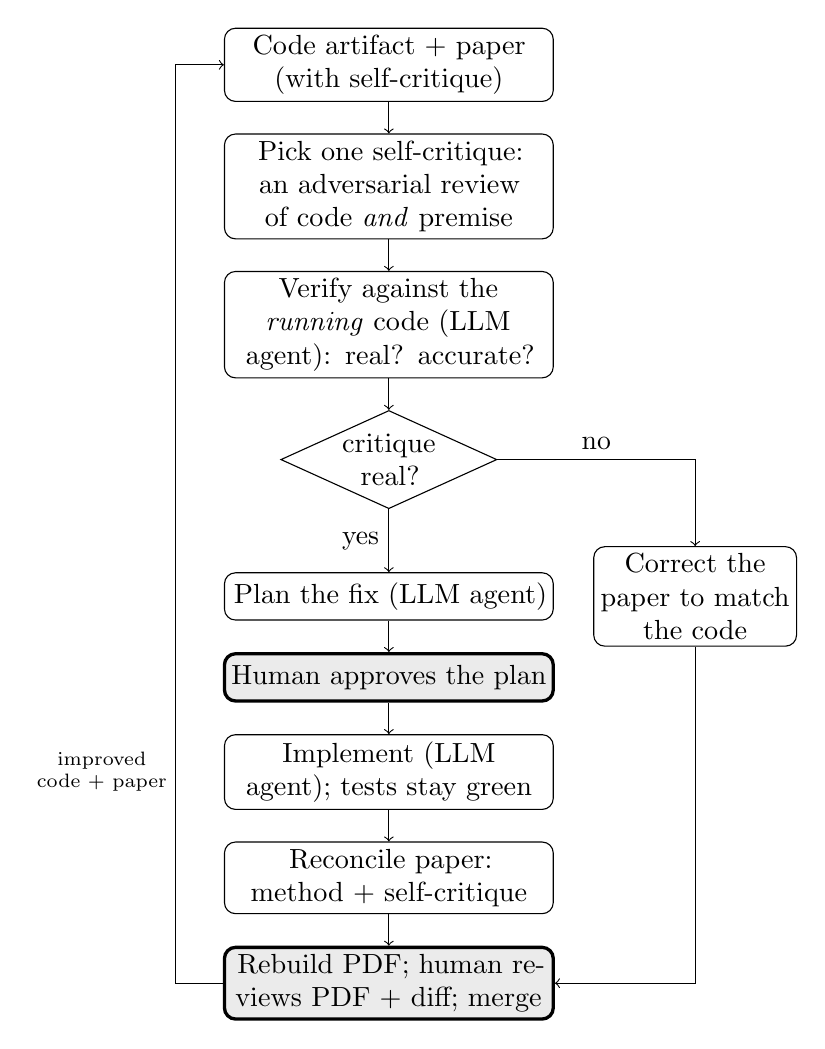
\begin{tikzpicture}[
  node distance=4mm,
  box/.style={draw, rounded corners, align=center, inner sep=2.5pt,
              text width=40mm, minimum height=6mm},
  gate/.style={box, fill=black!8, very thick},
  dec/.style={draw, diamond, aspect=2.2, align=center, inner sep=0pt,
              text width=13mm},
  every path/.style={draw, ->}
]
\node[box] (artifact) {Code artifact $+$ paper (with self-critique)};
\node[box, below=of artifact] (pick) {Pick one self-critique:\\an adversarial review of code \emph{and} premise};
\node[box, below=of pick] (verify) {Verify against the \emph{running} code (LLM agent): real? accurate?};
\node[dec, below=of verify] (real) {critique real?};
\node[box, below=8mm of real] (plan) {Plan the fix (LLM agent)};
\node[gate, below=of plan] (approve) {Human approves the plan};
\node[box, below=of approve] (impl) {Implement (LLM agent); tests stay green};
\node[box, below=of impl] (recon) {Reconcile paper: method $+$ self-critique};
\node[box, right=5mm of plan, text width=24mm] (correct) {Correct the paper to match the code};
\node[gate, below=of recon] (merge) {Rebuild PDF; human reviews PDF $+$ diff; merge};

\path (artifact) -- (pick);
\path (pick) -- (verify);
\path (verify) -- (real);
\path (real) -- node[left] {yes} (plan);
\path (real.east) -| node[above,pos=0.25] {no} (correct.north);
\path (plan) -- (approve);
\path (approve) -- (impl);
\path (impl) -- (recon);
\path (recon) -- (merge);
\path (correct) |- (merge);
\node[left=6mm of impl, align=center, font=\scriptsize] {improved\\code $+$ paper};
\path (merge.west) -- ++(-6mm,0) |- (artifact.west);
\end{tikzpicture}%
}
\caption{The \texttt{reconcile-critique} loop (\S\ref{sec:reflexive}): the paper's
self-critique drives revision of an \emph{executable} artifact. Two human gates
(shaded) bracket every change: plan approval and merge review.}
\label{fig:loop}
\end{figure}

The method above is not static; it is the current state of a deliberate revision
loop (Figure~\ref{fig:loop}) in which the paper and the implementation co-evolve
under human direction.
The tool was built first, as the concrete artifact this paper documents
(\S\ref{sec:impl}). Writing the paper then forced each assumption to be stated
precisely enough to attack, and the resulting self-critique (\S\ref{sec:threats})
became the \emph{driver} of subsequent change rather than a closing disclaimer:
each threat is read as an adversarial review of the code and of the premise behind
an axis.

A single pass takes one self-critique and first \emph{verifies it against the
running code}: does the weakness actually exist, and is it described accurately?
The pass then corrects the paper where it misstates the artifact, changes the
method and code to address a confirmed weakness, or does both. Any affected text
in \S\ref{sec:method} and \S\ref{sec:threats} is reconciled with the result. The work is
carried out with agentic coding assistants (the same class of tool this paper
measures) under a human-in-the-loop gate: an agent investigates and proposes a
plan; the human approves it before any code or prose is touched; an agent
implements; the test suite must stay green; the paper is rebuilt; and the human
reviews the rendered result and the diff before the change is accepted.

Two properties make this more than ordinary editing. First, the artifact is
\emph{executable}, so a critique of the premise is checkable: if the paper claims
the code does $X$, that is either true of the running code or it is a defect in one
of them, and the loop must resolve the disagreement rather than soften the wording.
Second, the process is \emph{reflexive} (a paper about the cost of supervising
agentic coding is itself produced by supervising agentic coding), so the authors
are incidentally $n{=}1$ subjects of the regime the index scores
(\S\ref{sec:threats}). The loop is made explicit because it, more than any single
threshold, provides the method's route to refinement: the index is built to be
falsified and revised, and \S\ref{sec:validation} states the external evidence
meant to drive later passes.

\section{Implementation}\label{sec:impl}
The method is realised in an open-source reference
implementation~\cite{acsrepo} that doubles as the proof of concept for this
paper: every axis, threshold, and the engagement weighting described here is
exactly what the released tool computes.\footnote{Source and documentation:
\url{https://github.com/sagium/ai-code-cognitive-stress}. The qualitative
behaviour described in this section was produced by the released code.} The Python
project reads only local files, performs no network I/O at any stage, and
writes a self-contained HTML report plus a machine-readable JSON sibling.
Per-day aggregates are cached keyed by source-file modification time, so metric
or weighting changes recompute from cache without re-parsing logs. Adding a new
coding tool is a single adapter implementing the event protocol; the aggregate,
metric, optimum, and rendering stages are tool-agnostic. The tool is private
by design: session transcripts frequently contain proprietary code and
secrets, so the generated artefacts are treated as similarly sensitive. The tool
never transmits them.

The implementation also provides two optional, local pathways toward the
multi-participant calibration of \S\ref{sec:validation}. The first is an
anonymized, consent-gated \emph{research export}: a per-user file of derived
daily metrics (and their components) with the timezone dropped and calendar
dates randomly shifted, which the operator may choose to upload manually; the
tool itself transmits nothing, preserving the privacy invariant. The export
also carries, for any day the operator chose to grade, an optional
self-reported felt-stress rating on a coarse three-level scale ($0$--$2$),
entered by a single action in the desktop companion and otherwise kept on the
operator's machine; the field is a small integer or null, so it adds no
identifying detail. The second is a population \emph{calibration} step that
pools such exports and proposes normalization ceilings and composite weights
that cover the observed range of work patterns. Both read and write only local
files. The calibration fits the axis \emph{scales} to the population
distribution and suggests weights from the redundancy among axes; where pooled
exports carry enough graded days, it additionally reports descriptive
correlations between each axis and the self-reported rating. It does not fit
weights to felt load, which requires a labeled sample pooled across many
participants (\S\ref{sec:validation}).

\section{Illustrative Example}\label{sec:example}
To make the axes concrete, this section reports one author's own data for a single month
(19 active workdays). This is emphatically an \emph{illustration of the
instrument}, not evidence of validity; $n{=}1$, the subject is an author, and
there is no ground-truth load measure here. Qualitatively, the
engagement-weighted CODL pulled composite scores down on days dominated by
background ``cooking'' sessions while leaving interruption-dominated days
largely unchanged, and the weighted peak $\mathrm{CODL}^{\star}$ separated a day
of genuine four-way \emph{active} supervision from a day with four sessions
merely open. This is the behaviour the design intends; whether it tracks
\emph{felt} load is exactly the open question of \S\ref{sec:validation}. That
unresolved criterion motivates the threats considered next.

\section{Threats to Validity and Self-Critique}\label{sec:threats}
The following challenges to the method are ordered roughly by severity.

\paragraph{Taskload is not workload.} Every axis is computed from objective event
streams; none measures felt experience. Objective and subjective workload can
dissociate. A low composite does not prove that the operator felt little strain,
and vice versa. The validated
subjective instrument is NASA-TLX~\cite{hart1988}. The method records an
optional, coarse felt-stress self-report that supplies an experience-sampling
criterion, and the calibration correlates the axes against it where enough
graded days accrue; until that correlation is established on an adequate sample,
the index remains an unvalidated proxy for the construct it names.

\paragraph{The supervisory-control analogy is borrowed, not established.}
Fan-out, neglect time, and attention demand were developed for UAV/robot
operators~\cite{cummings2008,crandall2007}. Their transfer to LLM oversight is
plausible because both involve one human time-sharing across semi-autonomous
processes, but unproven. LLM agents differ in failure modes, feedback latency,
and the verbal/code modality of interaction. Recent AI-coding studies give the
transfer partial, in-domain support: automation complacency and rising reliance
have been observed directly in professional software engineers using LLM
assistants~\cite{qian2024}, and informing software engineers that code is LLM-generated
measurably raises their NASA-TLX workload~\cite{tang2024}. These vary trust and
provenance rather than the supervisory fan-out the axes model, so they
corroborate the cognitive cost without yet validating the specific
fan-out/neglect-time constructs borrowed here.

\paragraph{The magnitude of $\beta$ is borrowed.} That a background locus
carries a positive, effortful, and
stress-inducing monitoring cost is supported in the relevant supervisory domain by the
supervisory-control and automation literature on out-of-the-loop operation,
vigilance, and complacency (\S\ref{sec:codl})~\cite{endsley1995,warm2008,parasuraman2010,eriksson2017}, a
regime far closer to agent supervision than the laboratory. What remains imported
is the \emph{magnitude}: the specific $15$--$20\%$ figure behind $\beta=0.20$
comes from prospective-memory and goal-priming
paradigms~\cite{smith2003,masicampo2011}, not from software supervision, so the
value is a defensible prior rather than a measurement. The true $\beta$ may differ
by person, task, and tool, and may not be constant within a day; recovering it
from data is a validation target (\S\ref{sec:validation}).

\paragraph{Equal composite weights are a placeholder.} No axis is asserted to
dominate, but equality should not be interpreted as an empirical result. Without calibration against
a criterion, the composite's absolute scale is arbitrary and only its
\emph{relative} movement within one person's history is meaningful. The weights
are a configuration parameter rather than a hard-coded constant, and the
implementation includes a population step that suggests data-fitted weights from
the redundancy among axes across pooled exports (\S\ref{sec:impl}). That
suggestion is \emph{unsupervised}: while the optional felt-stress self-report
lets the calibration report descriptive axis-to-felt-load correlations where
graded days accrue, fitting and validating weights against felt load needs a
labeled sample pooled across many participants, so equal weights remain the
default pending that supervised calibration
(\S\ref{sec:validation}).

\paragraph{The Closure Deficit's idle gap is a proxy for a parked loop.}
The axis scores \emph{resumption load}: idle gaps in a session's timeline where a
parked loop was picked back up, weighted by gap length (\S\ref{sec:closure}). This
makes it independent of concurrency: two days with identical $C(t)$ score
differently if one reloaded its loops cold and the other did not. The axis has
its own limitations, stated plainly. First, the gap is a \emph{proxy}: it is
genuine wall-clock dormancy (no event of any kind), so a long \emph{autonomous}
agent turn is correctly \emph{not} counted as a resume. A gap that ends only
because a single long-running tool call returned its result is also excluded: the
resume is read from whether the operator or model re-engaged rather than a tool
returning, so that span counts as the agent's own working time, not a parked loop.
The converse failure remains unobservable from the logs: stepping away while a
session is mid-turn, or leaving a session idle in the foreground, is
indistinguishable from a deliberate suspension. The upper bound $\theta$ is a proxy in the same
spirit: the logs record activity, not process liveness, so a gap at least $\theta$
long is read as the tool closed and the loop released, yet an operator who left
the tool genuinely open and idle that long is not distinguished from one who
closed it. Second, and most importantly, the
duration$\to$cost relationship this axis leans on was measured in the laboratory
over \emph{short} interruptions, seconds to about a minute~\cite{monk2008,altmann2002};
even the bounded gaps this axis scores, up to the close cutoff $\theta$, extrapolate
well beyond that regime. The field study of interrupted programming~\cite{parnin2011} is
the closest in-domain anchor that resumption is costly at the minutes-and-up scale,
but the specific severity curve $\sigma(r)=\min(1,r/\Delta)$ and the saturation
horizon $\Delta$ are a modeling choice, not a fitted function. Third, the three
constants (the resume threshold $\tau$, the horizon $\Delta$, and the daily
ceiling $K$) are citation-anchored priors, not values calibrated against felt
load; the ceiling in particular borrows Cowan's working-memory bound by analogy
rather than measurement. A retrieval-cue effect the method does \emph{not} model cuts the
other way and is worth noting: an agent transcript is itself a strong cue for
reconstructing a suspended goal~\cite{altmann2002}, so a resumed \emph{agent}
session may be cheaper to reload than the cue-free laboratory task the curve is
drawn from, meaning the axis, if anything, may over-state the cost of a resume.
The axis is defined on every active day and returns no value only when there
is no activity at all (\S\ref{sec:composite}).

\paragraph{Engagement is interaction-anchored by design.} Foreground is proxied
by proximity to the operator's own messages within a grace window $g$. Silent
engagement (reading, thinking, reviewing diffs without typing) leaves no message
event, so it earns no \emph{foreground} weight: while the session is live it still
counts at the background weight $\beta$, and counts nothing only once the tool is
closed (\S\ref{sec:codl}). What is out of scope by construction, rather than a
measurement gap (\S\ref{sec:method}), is total cognitive work: the index measures
the load \emph{driven by agent interaction}, not the operator's whole workload.
This omission tends to understate the operator's total cognitive load. A high
score therefore shows that agent supervision alone consumed substantial measured
capacity, while any unrecorded work adds demands that the index does not capture.
The principal bias in the other direction is that any
operator message (including a perfunctory acknowledgement) grants full
foreground weight for the whole window, so a trivial message can be over-weighted
by up to $g$. The $5$-minute grace is a default, not fitted; like $\beta$ it is a
configurable, auditable parameter rather than a hidden constant, and both the
value of engagement weighting and the sensitivity to $g$ are validation targets
(\S\ref{sec:validation}).

\paragraph{Cross-tool comparability is partial.} Each adapter maps its tool's
logs onto one shared event vocabulary (user and assistant messages, tool
invocations, tool results), so the axes consume semantically typed events rather
than raw, tool-specific log lines, and the quantities they are built from are
deliberately count-independent: CODL is a headcount of concurrently active
sessions, the Closure Deficit is wall-clock idle time, and the interruption rate
excludes routine tool calls entirely (\S\ref{sec:codl}, \S\ref{sec:closure}).
Two adapter-specific definitions that feed the axes directly remain only partly
comparable. First, a \emph{tool error} is whatever each tool chooses to record
as one, and that signal feeds the interruption rate, so tools that surface or
log failures differently are not on a common scale. Second, the boundary that
delimits one \emph{session} (and hence the concurrency headcount and the idle
gaps between resumes) is set per adapter, so two tools can partition the same
span of work into different numbers of streams. Because the index is
single-subject and per-operator, the practical concern is one operator mixing
tools on a single timeline rather than comparison across people. Aggregating those
streams without a shared error and session-boundary convention still risks
systematic bias, and establishing that convention is left to a multi-tool
sample.

\paragraph{Single subject and borrowed thresholds.} The capacity threshold
($\approx 4$~\cite{cowan2001}) and interruption ceiling ($10$/hour) are
literature values, not fitted to the population of agentic-coding software engineers, who
may differ. The illustrative behaviour comes from one author ($n{=}1$). The reference
implementation provides the machinery to move beyond this (an anonymized
per-user export and a population-calibration step that refits the ceilings to
the pooled distribution, \S\ref{sec:impl}). What remains is a multi-participant
sample in which each participant runs the private tool locally and only derived
metrics and optional grades are pooled. That step
calibrates the axis \emph{scales} to how the population actually behaves; it is
a distinct achievement from validating the thresholds against felt load, which
additionally requires the felt-stress self-report of \S\ref{sec:validation}.
The export carries that self-report for graded days, but validation needs it
pooled at sufficient scale; a population-fitted ceiling is otherwise
population-relative, not construct-validated. Until that labeled sample exists,
the thresholds remain borrowed and the evidence remains $n{=}1$
(\S\ref{sec:validation}).

\paragraph{Modelling and boundary choices.} One-minute sampling, the residual
over-approximation of liveness (a stream counts as open across a run even through
sub-$\theta$ idle, discounted to $\beta$ but not to zero), and timezone handling
are all defaults that could materially move scores for shift workers or bursty
users. Timezone is always the operator's own local zone and the tool is
single-subject by design, so cross-timezone teams are out of scope rather than a
threat to this index. The work window is inferred per operator from the
$p_{10}$--$p_{90}$ of message hours rather than fixed to a universal band,
which avoids assuming one schedule fits every operator but introduces its own
choices (the percentile edges, the hour rounding, and the five-date minimum
before inference engages) and
assumes that message timing tracks actual working hours; an operator who works
silently or messages at odd hours will get a skewed band, and inference falls
back to the fixed default during cold start. The additive off-hours load that
lets work past the band raise the composite is likewise built from explicit
priors ($+30$ points, saturating at $90$ engaged minutes; a $3$-hour early-start
grace on the band's lower edge), not measured penalties; the magnitudes could
over- or under-state the true cost of off-hours work (and the grace could
misclassify a habitual pre-dawn shift as outlier work or vice versa), so both
are targets for calibration. That load is anchored to \emph{interaction} (engaged
minutes within the grace of the operator's own messages), so it ignores
background sessions running while the operator is away and counts only active
supervision of the agent. Silent reading or review without typing, and the lack
of any ``rest day'' notion, are therefore out of scope by construction rather
than measurement gaps: the index targets the additional strain of \emph{agentic
coding} surfaced through interaction, not total work or work--life balance
(\S\ref{sec:method}). Additionally,
tool errors are attributed to the work window at the instant each was logged:
the per-day aggregate retains a timestamp for every errored tool result, so an
error fired outside the window adds nothing to the work-hour rate even when its
stream straddles the window edge, and a burst at one end of a stream is
attributed to that end rather than spread across its whole lifetime. The one
residual is the fallback for archive entries that carry only an error count with
no per-error timestamps: those errors are apportioned uniformly across the
stream's $[a_s,b_s]$ lifetime, a coarser attribution for bursty or
session-boundary activity.

\paragraph{Construct and causal claims.} ``Stress'' in the project name is
aspirational; the composite is a load index. No causal link to burnout outcomes
(e.g.\ MBI~\cite{maslach1981}) is claimed or shown; the index is offered as a
self-assessment proxy for the overload patterns \emph{associated} with burnout
risk, an early-warning aid, not a validated burnout measure. Reactivity is also
possible: surfacing the score may itself change behaviour. And because the index
covers only coding-agent interaction (\S\ref{sec:method}), it is silent on total
workload: a low score does not certify a sustainable day, only a light
\emph{agent-supervision} load. Symmetrically, the finite-budget reading (that a
heavy supervision load leaves less capacity for the rest of an engineer's
role) is an interpretation the index invites, not one it measures: it never
observes the non-coding work, so any crowd-out there is a hypothesis for
validation (\S\ref{sec:validation}), not a reported result.

\section{Falsifiable Predictions and Validation Roadmap}\label{sec:validation}
Together, the critiques above define a research agenda. The following predictions
make the design falsifiable.

\begin{enumerate}
  \item \textbf{Concurrent validity.} Across a sample of agentic-coding
  software engineers, daily composite should correlate positively with same-day
  NASA-TLX~\cite{hart1988} or ecological momentary assessments of effort. A null
  or negative correlation falsifies the composite as a load proxy.
  \item \textbf{Structure beats volume.} The three axes should predict felt
  load (and the capacity crowd-out below) \emph{better than raw
  agent-interaction time alone}. If total supervision minutes predict equally
  well, the decomposition into fan-out, interruption, and closure adds no
  information over a stopwatch and should be simplified.
  \item \textbf{Capacity crowd-out.} On days whose agent-supervision load is
  extreme, the non-coding work the role also requires (design, review,
  coordination) should measurably suffer: lower self-rated capacity for it,
  reduced throughput or quality, or its displacement into off-hours. Absence of
  any such spillover would mean a heavy supervision load does not in fact compete
  for a shared budget, narrowing the index to a within-activity measure.
  \item \textbf{Engagement-weighting ablation.} Engagement-weighted CODL should
  correlate with felt load \emph{better} than the flat headcount. If weighting
  does not improve the correlation, $\beta$ and $g$ add complexity without value.
  \item \textbf{Weight calibration.} Regressing subjective load on the three
  normalized axes should yield weights that beat the equal-weight null
  out-of-sample; the fitted weights would become candidate defaults. The
  implementation derives \emph{unsupervised}, redundancy-based weight
  suggestions from pooled exports and, where graded days accrue, reports
  descriptive axis-to-felt-load correlations (\S\ref{sec:impl}); this prediction
  concerns the \emph{supervised} step beyond those descriptives: fitting and
  validating weights against the felt-load criterion on a labeled
  multi-participant sample.
  \item \textbf{Predictive validity for recovery.} Days high in off-hours
  activity and composite should predict lower next-day vigor/detachment
  scores~\cite{sonnentag2010}; absence of this relationship weakens the recovery
  framing.
  \item \textbf{$\beta$ recovery from data.} With per-event timestamps and a
  secondary signal (e.g.\ self-reported ``which sessions were you actually
  watching''), $\beta$ can be estimated rather than assumed; the estimate's
  distance from $0.20$ quantifies the prior's error.
  \item \textbf{Sensitivity analysis.} Composite rankings of days should be
  stable under reasonable perturbations of $g$, the sampling interval, and the
  thresholds; instability would indicate over-tuned, non-robust scoring.
  \item \textbf{Inferred window vs.\ fixed band.} The per-operator inferred
  window should predict felt load (or in-flow time) better than the fixed
  09:00--19:00 band out-of-sample. If inference does not beat the fixed band,
  the percentile machinery adds complexity without value and the fixed default
  should be preferred.
  \item \textbf{Off-hours load validity.} Days carrying a high off-hours
  engaged-minutes load should predict lower next-day vigor/detachment~\cite{sonnentag2010};
  if the load does not track reduced recovery, its magnitude
  ($+30$ points, $90$-minute saturation) is mis-specified and should be
  refit or dropped.
  \item \textbf{Population threshold check.} With multi-participant data, the
  $\approx 4$ capacity ceiling~\cite{cowan2001} and $10$/hour interruption
  ceiling can be checked and, if warranted, refit to the agentic-coding
  population; large divergence would mean the borrowed values mis-set the axis
  scales. The calibration step computes exactly this from pooled exports
  (\S\ref{sec:impl}); what remains is collecting the population.
\end{enumerate}
A modest multi-participant study with experience sampling is the primary
outstanding work. Each participant would run the private tool locally, with only
derived daily metrics and subjective ratings pooled for analysis. The released
tooling supports this design through the anonymized export and pooled-calibration
step (\S\ref{sec:impl}), without adding an off-machine data path to the tool.
Such a study would address most threats in \S\ref{sec:threats}, especially the
single-subject evidence and borrowed thresholds, and determine whether the
principled instrument is also a valid one.
On the closure side, the outstanding work is calibrating the resume threshold,
decay horizon, and daily ceiling against felt load rather than borrowing them
(\S\ref{sec:closure}), and better separating a deliberately parked loop from an
idle foreground session.

\section{Ethics and Privacy}
The validation design depends on protecting the source material from which the
metrics are derived. Session logs can contain proprietary source code and
secrets; private processing is therefore treated as a hard invariant, not a
feature, and any future
data-sharing path would require separate, explicit, opt-in consent. The intended
use is individual self-reflection. This work explicitly warns against managerial or
comparative use across people: the index is calibrated to an individual's own
history, the construct is unvalidated, and using an unvalidated load proxy for
evaluation would be both statistically and ethically unsound.

\section{Conclusion}
Agentic coding and multi-agent orchestration have created an emerging and largely
unmeasured cognitive regime: one engineer supervising many semi-autonomous
processes at machine pace. The central problem is to find the sustainable pace at
which throughput gains and supervision quality can both be maintained. This work
has presented a local, privacy-preserving, literature-anchored method for making the
\emph{behavioural} footprint of that regime visible to the individual who
generates it, including an engagement-weighted concurrency measure that
distinguishes active supervision from background agent work. The analysis also
states what the method does not yet establish and sets out falsifiable
predictions and a validation path.

Nothing in the three axes is specific to programming. Working-memory
capacity~\cite{cowan2001}, attention residue from
interruption~\cite{leroy2009,mark2008}, the monitoring cost of an open
loop~\cite{smith2003,masicampo2011}, and the demands--resources balance that
governs recovery~\cite{demerouti2001,mcewen1998} are properties of the human
operator, not of the work being supervised; the only domain-specific part of the
pipeline is the input adapter that turns one tool's session logs into typed
events (\S\ref{sec:impl}). Supervising a set of semi-autonomous agents is
becoming a common form of knowledge work, and software engineering is an early
case because this form of automation reached it early. As other
professions take on the same supervisory relationship, similar concurrency,
interruption, and closure load may surface. Like the rest of the construct,
this generalization is an empirical claim to be tested rather than assumed
(\S\ref{sec:validation}).

The explicit assumptions and open implementation make the construct easy to
challenge. That scrutiny is essential to making both the construct and any tool
built on it more trustworthy.
The index is offered as a self-regulating signal: each engineer closes
the loop between the throughput gains agentic tools offer and the sustainable pace
at which those gains can be maintained without degrading the supervision that makes
them valuable.

\bibliographystyle{plain}
\bibliography{references}

\end{document}
